% Author: Izaak Neutelings (March 2020)
\documentclass[border=3pt,tikz]{standalone}
\usepackage{amsmath} % for \dfrac
\usepackage{mathabx} % for \Earth
\usepackage{bm} % \bm
\usepackage{physics}
\usepackage{tikz}
\usetikzlibrary{angles,quotes} % for pic (angle labels)
\usetikzlibrary{arrows.meta}
\usetikzlibrary{calc}
\usetikzlibrary{decorations.markings}
\tikzset{>=latex} % for LaTeX arrow head
\usepackage{xcolor}
\colorlet{Bcol}{violet!90}
\colorlet{BFcol}{red!50!black}
\colorlet{vcol}{red!50!black}
\colorlet{veccol}{green!50!black}
\colorlet{Icol}{blue!70!black}
\colorlet{wcol}{orange!90!black}
\colorlet{metal}{blue!30!black!12}
\colorlet{Scol}{green!60!black}
\tikzstyle{BField}=[->,very thick,Bcol]
\tikzstyle{current}=[->,Icol] %thick,
\tikzstyle{force}=[->,very thick,BFcol]
\tikzstyle{velocity}=[->,thick,vcol]
\tikzstyle{spin}=[->,very thick,Scol]
\tikzstyle{charge+}=[very thin,draw=black,top color=red!50,bottom color=red!90!black,shading angle=20,circle,inner sep=0.2]
\tikzstyle{charge-}=[very thin,draw=black,top color=blue!50,bottom color=blue!80,shading angle=20,circle,inner sep=0.2]
\tikzstyle{vector}=[->,thick,veccol]
\tikzset{
  BFieldLine/.style={thick,Bcol,decoration={markings,mark=at position #1 with {\arrow{latex}}},
                     postaction={decorate}},
  BFieldLine/.default=0.5,
  pics/Bin/.style={
    code={
      \def\RB{0.12}
      \draw[pic actions,#1,line width=0.6] % ,thick
        (0,0) circle (\RB) (-135:.7*\RB) -- (45:.7*\RB) (-45:.7*\RB) -- (135:.7*\RB);
  }},
  pics/Bout/.style={
    code={
      \def\RB{0.12}
      \draw[pic actions,#1,fill=white,line width=0.6] (0,0) circle (\RB);
      \fill[pic actions,#1] (0,0) circle (0.3*\RB);
  }},
  pics/Bout/.default=Bcol,
  pics/Bin/.default=Bcol,
  pics/spin/.style={
    code={
      \def\L{0.38}
      \draw[-{Latex[length=3,width=2.5]},pic actions,rotate=#1,line width=0.8,Scol] (0,0) -- (\L,0);
      \draw[pic actions,rotate=#1,thin,white]
        (0.35*\L,0)++(170:{0.16*\L} and {0.22*\L}) arc (170:190:{0.16*\L} and {0.22*\L});
      \draw[-{Latex[length=1.2,width=1]},pic actions,rotate=#1,very thin]
        (0.35*\L,0)++(25:{0.16*\L} and {0.22*\L}) arc (25:305:{0.16*\L} and {0.22*\L}) --++ (50:0.09*\L);
  }},
  pics/spin/.default=90,
}



\begin{document}


% CYCLOTRON FREQUENCY
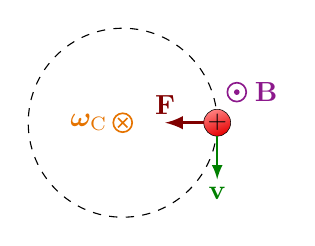
\begin{tikzpicture}
  \def\R{1.2}
  \def\v{0.6*\R}
  \def\F{0.55*\R}
  \coordinate (O) at (0,0);
  \coordinate (Q) at (\R,0);
  
  % MAGNETIC FIELD
  %\foreach \i [evaluate={\y=(\i-1)*\ymax/(\NBy-1);}] in {1,...,\NBy}{
  %  \foreach \i [evaluate={\x=(\i-1)*\xmax/(\NBx-1);}] in {1,...,\NBx}{
  %    \pic[rotate=-90] at (\x,\y) {Bin};
  %  }
  %}
  \pic at (15:1.25*\R) {Bout};
  \node[Bcol,right=3] at (15:1.25*\R) {$\vb{B}$};
  
  % ROTATION VECTOR
  \pic at (O) {Bin={wcol}};
  \node[wcol,left=2] at (O) {$\vb*{\omega}_\mathrm{C}$};
  
  % CHARGE
  \draw[dashed] (O) circle (\R);
  \node[charge+,scale=0.9] (Q) at (Q) {$+$};
  \draw[vector] (Q) --++ (-90:\v) node[below=-1] {$\vb{v}$};
  \draw[force] (Q) --++ (180:\F) node[above=-1] {$\vb{F}$};
  
\end{tikzpicture}


% CYCLOTRON FREQUENCY, negative
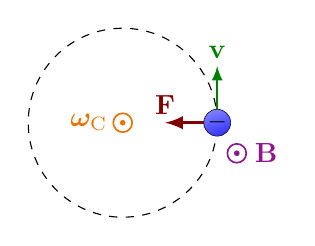
\begin{tikzpicture}
  \def\R{1.2}
  \def\v{0.6*\R}
  \def\F{0.55*\R}
  \coordinate (O) at (0,0);
  \coordinate (Q) at (\R,0);
  
  % MAGNETIC FIELD
  %\foreach \i [evaluate={\y=(\i-1)*\ymax/(\NBy-1);}] in {1,...,\NBy}{
  %  \foreach \i [evaluate={\x=(\i-1)*\xmax/(\NBx-1);}] in {1,...,\NBx}{
  %    \pic[rotate=-90] at (\x,\y) {Bin};
  %  }
  %}
  \pic at (-15:1.25*\R) {Bout};
  \node[Bcol,right=3] at (-15:1.25*\R) {$\vb{B}$};
  
  % ROTATION VECTOR
  \pic at (O) {Bout={wcol}};
  \node[wcol,left=2] at (O) {$\vb*{\omega}_\mathrm{C}$};
  
  % CHARGE
  \draw[dashed] (O) circle (\R);
  \node[charge-,scale=0.9] (Q) at (Q) {$-$};
  \draw[vector] (Q) --++ (90:\v) node[above=-1] {$\vb{v}$};
  \draw[force] (Q) --++ (180:\F) node[above=-1] {$\vb{F}$};
  
\end{tikzpicture}


% CYCLOTRON g = 2
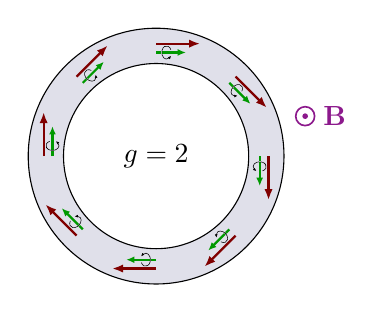
\begin{tikzpicture}
  \def\R{1.4}
  \def\v{0.4*\R}
  \def\F{0.55*\R}
  \def\N{8}
  \coordinate (O) at (0,0);
  \coordinate (Q) at (\R,0);
  
  % CYCLOTRON
  \draw[fill=metal,even odd rule] (O) circle (0.84*\R) circle (1.16*\R);
  
  % MAGNETIC FIELD
  \pic at (15:1.4*\R) {Bout};
  \node[Bcol,right=3] at (15:1.4*\R) {$\vb{B}$};
  
  % SPINS
  \foreach \i [evaluate={\ang=90-(\i-1)*360/\N;}] in {1,...,\N}{
    \draw[velocity,-{Latex[length=4,width=3]}] (\ang:1.02*\R) --++ (\ang-90:\v);
    \pic at (\ang:0.94*\R) {spin={\ang-90}};
  }
  \node at (0,0) {$g = 2$};
  
\end{tikzpicture}


% ANOMALOUS PRECESSION
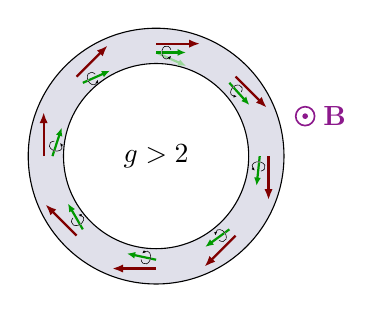
\begin{tikzpicture}
  \def\R{1.4}
  \def\v{0.4*\R}
  \def\F{0.55*\R}
  \def\N{8}
  \coordinate (O) at (0,0);
  \coordinate (Q) at (\R,0);
  
  % CYCLOTRON
  \draw[fill=metal,even odd rule] (O) circle (0.84*\R) circle (1.16*\R);
  
  % MAGNETIC FIELD
  \pic at (15:1.4*\R) {Bout};
  \node[Bcol,right=3] at (15:1.4*\R) {$\vb{B}$};
  
  % SPINS
  \draw[-{Latex[length=3,width=2.5]},thick,Scol!40] (90:0.94*\R) --++ (-3*\N:0.30*\R);
  \foreach \i [evaluate={\ang=90-(\i-1)*360/\N; \dang=3*(\i-1);}] in {1,...,\N}{
    \draw[velocity,-{Latex[length=4,width=3]}] (\ang:1.02*\R) --++ (\ang-90:\v);
    \pic at (\ang:0.94*\R) {spin={\ang-90-\dang}};
  }
  \node at (0,0) {$g > 2$};
  
\end{tikzpicture}


% ANOMALOUS PRECESSION
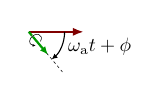
\begin{tikzpicture}
  \def\v{0.7}
  \def\N{8}
  \def\ang{-50}
  \coordinate (O) at (0,0);
  
  % SPINS
  \draw[very thin,dash pattern=on 1pt off 1pt] (O) -- (\ang:0.95*\v);
  %\draw[-{Latex[length=3,width=2.5]},thick,Scol!40] (90:0.94*\R) --++ (-3*\N:0.30*\R);
  \draw[velocity,-{Latex[length=4,width=3]}] (O) --++ (\v,0);
  \pic[scale=1] at (O) {spin={\ang}};
  %\draw[-{Latex[length=2,width=2]},scale=0.5]
  %  (\ang-30:0.8*\v) arc (\ang-30:\ang-100:0.8*\v)
  %  node[midway,below,scale=0.8] {$\omega_\mathrm{a}$};
  \draw[-{Latex[length=2,width=2]}]
    (0:0.65*\v) arc (0:\ang:0.65*\v)
    node[midway,right,scale=0.7] {$\omega_\mathrm{a}t + \phi$};
  
\end{tikzpicture}



% ANOMALOUS PRECESSION - 10
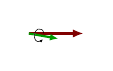
\begin{tikzpicture}
  \def\v{0.7}
  \def\ang{-10}
  \coordinate (O) at (0,0);
  \draw[velocity,-{Latex[length=4,width=3]}] (O) --++ (\v,0);
  \pic[scale=1] at (O) {spin={\ang}};  
\end{tikzpicture}



% ANOMALOUS PRECESSION - 50
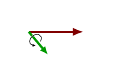
\begin{tikzpicture}
  \def\v{0.7}
  \def\ang{-50}
  \coordinate (O) at (0,0);
  \draw[velocity,-{Latex[length=4,width=3]}] (O) --++ (\v,0);
  \pic[scale=1] at (O) {spin={\ang}};  
\end{tikzpicture}



% ANOMALOUS PRECESSION - 120
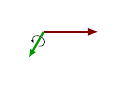
\begin{tikzpicture}
  \def\v{0.7}
  \def\ang{-120}
  \coordinate (O) at (0,0);
  \draw[velocity,-{Latex[length=4,width=3]}] (O) --++ (\v,0);
  \pic[scale=1] at (O) {spin={\ang}};  
\end{tikzpicture}



% ANOMALOUS PRECESSION - 150
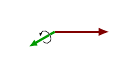
\begin{tikzpicture}
  \def\v{0.7}
  \def\ang{-150}
  \coordinate (O) at (0,0);
  \draw[velocity,-{Latex[length=4,width=3]}] (O) --++ (\v,0);
  \pic[scale=1] at (O) {spin={\ang}};  
\end{tikzpicture}



\end{document}
